\section{Logistic Regression \& Softmax}
\begin{frame}{Adapting Linear Regression for Classification}
    \begin{columns}[c]
        \begin{column}{1.0\textwidth}
            \textbf{The Challenge:}
            We want to classify data (e.g., Spam vs Not Spam).
            
            \vspace{1em}
            However, our Linear Model $f(x) = \mathbf{w}^T\mathbf{x}$ outputs numbers in $(-\infty, \infty)$.
            
            \vspace{1em}
            \begin{exampleblock}{Problem}
                If model outputs $500$ or $-20$, how do we interpret that as a probability?
            \end{exampleblock}
            
            \vspace{1em}
            We need a mechanism to map these raw "scores" into a valid probability range $[0, 1]$.
        \end{column}
    \end{columns}
\end{frame}

% --- Slide 2: The Workflow Visualization (New) --
% Define some nicer colors
\definecolor{myblue}{RGB}{70,130,180}
\definecolor{myred}{RGB}{220,50,50}
\definecolor{myorange}{RGB}{255,140,0}
\definecolor{mygreen}{RGB}{60,179,113}

\begin{frame}{The Classification Pipeline}

\centering
\resizebox{1.0\linewidth}{!}{
\begin{tikzpicture}[
    node distance=1.8cm,
    every node/.style={font=\sffamily},
    % --- Clean, Professional Box Style (Grayscale) ---
    vectorBox/.style={
        rectangle, 
        rounded corners=3pt, 
        draw=gray!40, 
        line width=1pt, 
        top color=white, 
        bottom color=gray!5, 
        align=center,
        drop shadow={opacity=0.15, shadow xshift=1pt, shadow yshift=-1pt},
        inner sep=6pt, 
        minimum height=3.2cm, 
        minimum width=1.5cm
    },
    % --- Output Circle Style ---
    circleBox/.style={
        circle, 
        draw=gray!40, 
        line width=1pt, 
        top color=white, 
        bottom color=gray!5, 
        align=center,
        drop shadow={opacity=0.15}, 
        minimum size=2.2cm, 
        font=\sffamily\bfseries\large
    },
    % --- Arrow Styles ---
    % 1. Boring gray arrows for normal flow
    stdArrow/.style={-{Latex[length=2.5mm, width=1.5mm]}, thick, gray!50},
    % 2. HIGHLIGHT arrow (Orange) - Pops out but looks pro
    highlightArrow/.style={-{Latex[length=3mm, width=2mm]}, line width=2pt, orange!80!red},
    % --- Label Styles ---
    arrowLbl/.style={font=\footnotesize\sffamily, text=gray!80, align=center, inner sep=3pt},
    highlightLbl/.style={font=\footnotesize\sffamily\bfseries, text=orange!80!red, align=center, inner sep=3pt}
]

    % --- 1. Inputs ---
    \node[vectorBox] (input) {
        \textbf{Inputs}\\[0.5em]
        $x_1$\\$x_2$\\$\vdots$\\$x_d$
    };

    % --- 2. Scores ---
    \node[vectorBox, right=of input] (logits) {
        \textbf{Scores}\\[0.5em]
        $0.5$\\$12.2$\\$-3.1$\\$\vdots$
    };

    % Arrow 1 (Standard)
    \draw[stdArrow] (input) -- 
        node[above, arrowLbl] {Linear Model} 
        node[below=1pt, arrowLbl] {$\mathbf{w}^T\mathbf{x}$} 
        (logits);

    % --- 3. Probs ---
    \node[vectorBox, right=of logits] (probs) {
        \textbf{Probs}\\[0.5em]
        $0.62$\\$0.99$\\$0.04$\\$\vdots$
    };

    % Arrow 2 (THE HIGHLIGHT)
    \draw[highlightArrow] (logits) -- 
        node[above, highlightLbl] {Special\\Function} 
        node[below=1pt, highlightLbl, font=\footnotesize\itshape] {$\sigma(\mathbf{w}^T\mathbf{x})$} 
        (probs);

    % --- 4. Output ---
    \node[circleBox, right=of probs] (output) {
        Class\\0 or 1
    };

    % Arrow 3 (Standard)
    \draw[stdArrow] (probs) -- 
        node[above, arrowLbl] {Threshold} 
        node[below=1pt, arrowLbl] {$> 0.5?$} 
        (output);

\end{tikzpicture}
}
\end{frame}


% --- Slide 3: The Solution (Sigmoid) ---
\begin{frame}{The Solution: The Sigmoid Function}
    The "Special Function" we need is the \textbf{Sigmoid} (Logistic Function).
    
    \begin{columns}[c]
        \begin{column}{0.45\textwidth}
            \begin{tcolorbox}[colback=blue!5, title=\textbf{Sigmoid Function}]
                \vspace{-1em}
                $$ \hat{y} = \sigma(z) = \frac{1}{1 + e^{-z}} $$
            \end{tcolorbox}
            
            \textbf{Properties:}
            \begin{itemize}
                \item Squashes any $z$ into $(0, 1)$.
                \item $z=0 \implies \hat{y}=0.5$.
                \item Differentiable everywhere (Smooth).
            \end{itemize}
        \end{column}
        
        \begin{column}{0.55\textwidth}
            \centering
            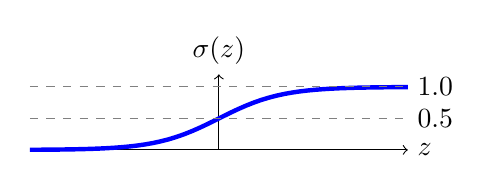
\begin{tikzpicture}[scale=0.8]
                \draw[->] (-3,0) -- (3,0) node[right] {$z$};
                \draw[->] (0,0) -- (0,1.2) node[above] {$\sigma(z)$};
                % Sigmoid
                \draw[blue, ultra thick, domain=-3:3, samples=50] plot (\x, {1/(1+exp(-\x*2))});
                % Limits
                \draw[dashed, gray] (-3,1) -- (3,1) node[right, black] {1.0};
                \draw[dashed, gray] (-3,0.5) -- (3,0.5) node[right, black] {0.5};
            \end{tikzpicture}
        \end{column}
    \end{columns}
\end{frame}

% --- Slide 4: Gradient Derivation Part 1 ---
\begin{frame}{The Gradient: Chain Rule Breakdown}
    To train, we need to minimize the Binary Cross-Entropy Loss:
    $$ J = - [y \log(\hat{y}) + (1-y) \log(1-\hat{y})] $$

    Let's compute $\frac{\partial J}{\partial w}$ using the Chain Rule:
    $$ \frac{\partial J}{\partial w} = \textcolor{red}{\frac{\partial J}{\partial \hat{y}}} \cdot \textcolor{blue}{\frac{\partial \hat{y}}{\partial z}} \cdot \textcolor{green!60!black}{\frac{\partial z}{\partial w}} $$

    \vspace{1em}
    \textbf{The Three Components:}
    \begin{enumerate}
        \item \textcolor{red}{\textbf{Loss Derivative:}} $\frac{\hat{y} - y}{\hat{y}(1-\hat{y})}$
        \item \textcolor{blue}{\textbf{Sigmoid Derivative:}} $\hat{y}(1-\hat{y})$ \hfill \textit{(Can you derive this?)}
        \item \textcolor{green!60!black}{\textbf{Linear Derivative:}} $x$
    \end{enumerate}
\end{frame}

% --- Slide 5: Gradient Derivation Part 2 ---
\begin{frame}{The Gradient "Magic"}
    Now, multiply them together:
    
    $$ \frac{\partial J}{\partial w} = \left( \frac{\hat{y} - y}{\cancel{\hat{y}(1-\hat{y})}} \right) \cdot \cancel{\hat{y}(1-\hat{y})} \cdot x $$
    
    The complicated Sigmoid derivative perfectly cancels the denominator of the Log Loss!

    \begin{tcolorbox}[colback=green!5, title=\textbf{Final Gradient Update}]
        $$ \nabla J(\mathbf{w}) = \frac{1}{N} \mathbf{X}^T (\mathbf{\hat{y}} - \mathbf{y}) $$
    \end{tcolorbox}
    
    \begin{tcolorbox}[colback=yellow!10, colframe=orange!50, title=\textbf{Observation}]
        This formula is \textbf{identical} to Linear Regression (ignore constants)!
        The only difference is how we calculate $\hat{y}$ (Sigmoid vs. Identity).
    \end{tcolorbox}
\end{frame}

\begin{frame}{Generalization: Multiclass (Softmax)}
    What if we have $K > 2$ classes? (e.g., Cat, Dog, Bird).
    We generalize Sigmoid to \textbf{Softmax}.

    \vspace{0.5em}
    \begin{columns}[T]
        \begin{column}{0.5\textwidth}
            \begin{tcolorbox}[colback=blue!5, colframe=blue!50!black, title=\textbf{Softmax Function}]
            \vspace{-1em}
                $$ P(y=k) = \frac{e^{z_k}}{\sum_{j=1}^{K} e^{z_j}} $$
            \end{tcolorbox}
            
            \small
            \begin{itemize}
                \item \textbf{Exponent ($e^z$):} Forces all scores to be positive.
                \item \textbf{Sum ($\sum$):} Normalizes so all probabilities sum to $1.0$.
                \item \textbf{Loss:} Cross-Entropy.
                $$
                J = - \frac{1}{n}\sum_{i=1}^{n}
                \sum_{k=1}^{K}
                y_{i,k}\log(\hat{y}_{i,k})
                $$
            \end{itemize}
        \end{column}
        
        \begin{column}{0.45\textwidth}
    \centering
    \scalebox{0.9}{ 
    \begin{tikzpicture}[
        % Tighter vertical spacing
        node distance=0.6cm and 0.5cm, 
        every node/.style={font=\sffamily},
        % Styles for the boxes
        box/.style={
            rectangle, 
            rounded corners=3pt, 
            draw=gray!30, 
            line width=0.8pt,
            top color=white, 
            bottom color=gray!5, 
            align=center,
            drop shadow={opacity=0.1, shadow xshift=1pt, shadow yshift=-1pt},
            inner sep=5pt % Reduced padding
        },
        % Style for the function box
        func/.style={
            rectangle, 
            rounded corners=3pt, 
            draw=blue!30, 
            fill=blue!5, 
            thick, 
            align=center, 
            inner sep=6pt, % Reduced padding
            drop shadow={opacity=0.1, shadow xshift=1pt, shadow yshift=-1pt}
        },
        arrow/.style={-{Latex[length=2.5mm, width=1.5mm]}, thick, gray!60},
        lbl/.style={font=\scriptsize\itshape, text=gray!80, anchor=west}
    ]

        % --- 1. Logits Node ---
        \node[box] (z) {
            \textbf{\small Scores ($z$)} \\[0.2em]
            \begin{tabular}{r l}
                \textcolor{red!80!black}{\textbf{2.0}} & \scriptsize (Cat) \\
                1.0 & \scriptsize (Dog) \\
                0.1 & \scriptsize (Bird)
            \end{tabular}
        };
        \node[lbl, right=0.1cm of z.east] {Raw Logits};

        % --- 2. Softmax Function Node ---
        \node[func, below=of z] (softmax) {
            $\displaystyle \sigma(z)_i = \frac{e^{z_i}}{\sum_{j} e^{z_j}}$
        };

        % --- 3. Probabilities Node ---
        \node[box, below=of softmax] (p) {
            \textbf{\small Probs ($P$)} \\[0.2em]
            \begin{tabular}{r l}
                \textcolor{blue!80!black}{\textbf{0.66}} & \scriptsize (Cat) \\
                0.24 & \scriptsize (Dog) \\
                0.10 & \scriptsize (Bird)
            \end{tabular}
        };
        \node[lbl, right=0.1cm of p.east] {$\sum = 1.0$};

        % --- Arrows ---
        \draw[arrow] (z) -- (softmax);
        \draw[arrow] (softmax) -- (p);

    \end{tikzpicture}
    } % End of scalebox
\end{column}
    \end{columns}
\end{frame}


% --- Slide: Pros & Cons of Linear Models ---
\begin{frame}{Linear Models: Advantages \& Disadvantages}
    \begin{columns}[T]
        % PROS
        \begin{column}{0.48\textwidth}
            \begin{tcolorbox}[colback=green!5, title=Advantages]
                \begin{itemize}
                    \item \textbf{Interpretable:} The weights $\mathbf{w}$ directly tell us feature importance.
                    \item \textbf{Fast \& Efficient:} Training is simple matrix math. Inference is just a dot product.
                \end{itemize}
            \end{tcolorbox}
        \end{column}

        % CONS
        \begin{column}{0.48\textwidth}
            \begin{tcolorbox}[colback=red!5, title=Disadvantages]
                \begin{itemize}
                    \item \textbf{High Bias (Underfitting):} Cannot model complex, non-linear relationships.
                    \item \textbf{Sensitive to Outliers.} Especially when using MSE.
                    \item \textbf{Scaling Required:} Sensitive to feature magnitude (Requires Standardization).
                \end{itemize}
            \end{tcolorbox}
        \end{column}
    \end{columns}

\end{frame}


% --- Custom Colors ---
\definecolor{myblue}{RGB}{70,130,180}
\definecolor{mygreen}{RGB}{60,179,113}
\definecolor{myred}{RGB}{220,50,50}
\definecolor{myorange}{RGB}{255,140,0}

% ==============================================================================
% SECTION 2: DISTANCE-BASED (K-NN)
% ==============================================================================

\subsection{Distance-Based Models}

% --- Roadmap: Moving to Distance-Based ---
